\section{EXPERIMENTAL STUDY}

\added{The empirical} \deleted{Empirical} research presented in this \deleted{experimental} aims to evaluate the combination
of well-known semi-automatic (software visualization) and automatic (data clustering) techniques in the context of a 
software architecture recovery to understand the modular decomposition of a system. \replaced{We guided our study}{The study was performed} using the 
Goal Question Metric (GQM) approach, as described in Table~\ref{tab:RecoveryTechniques}.

\begin{table}
	\centering
	\caption{Definition of the accuracy evaluation Software Architecture Recovery Techniques.}
	\resizebox{\columnwidth}{!}{%
	\begin{tabular}{@{}ll@{}}
		\toprule
		\textbf{Purpose}   & Evaluate    \\
		\textbf{Issue}     & accuracy of the modular decomposition \\
		\textbf{Object}    & architecture recovery using semi-automatic and automatic techinques\\
		\textbf{Viewpoint} & software architect / application engineer\\
		\textbf{Context}   & University of Brasilia Academic Management Systems		              \\ \bottomrule
	\end{tabular}
	}
	\label{tab:RecoveryTechniques}
\end{table}

The underlying research question for this experiment is as follows: 
\emph{Does the use of software visualization technique, along with the clustering technique, increases the 
accuracy of the architectural model produced, in comparison with using only one of the techniques?}
 
Each participant recovered the architecture by 
applying two reengineering approaches per session, which produced two models 
representing de modular decomposition of the system. 
In the first session, the participant 
applied only one technique using either a semi-automatic decomposition 
based on software visualization or an automatic decomposition 
based on software clustering. 
After obtaining the first model, the other approach was presented and 
it was requested to produce a new model, based on the two techniques. 
In this way it was possible 
to calculate the accuracy of the resulting models.

To calculate the accuracy of the recovered architectural representation of the modular decomposition 
of the systems, and then answering the questions of the experiment, we used the 
Jaccard similarity coefficient, defined by the formula:

\begin{center}
	$Sj= \frac{a}{a+b+c}$
\end{center}

Here: $Sj$ is the coefficient of Jaccard; $a$= the number of common receovered 
modules; $b$= number of modules recovered in B but not in A; $c$= number of recovered 
modules in A, but not in B. In the experiment, model B was produced by a domain expert, while the model 
A was produced by \added{the}participants \replaced{of}{in} the experiment.

\subsection{Design}%

This section presents the experimental design of 
this research, in a level of details that might help other researchers to replicate 
our study~\cite{Juristo_2010} using a similar setting.

%% \deleted{This section describes the experiment plan 
%% and demonstrates how 
%% the experiment was designed. This allows the execution of 
%% other studies based on the same plan~\cite{Juristo_2010}.}

The study considered four software systems, written in 
two programming languages (Visual Basic and Java).
Table \ref{tabelaSistemasObjetos}  presents relevant information on 
the characteristics of each object of the experiment. Systems A 
and B are legacy systems still operating in the University of Brasilia, 
and both support the management of the academic routine of college students. 
Systems C and D have been developed on a new platform, in order 
to modernize legacy systems written in Visual Basic. These systems 
deal with administrative university routines.

\begin{table}[h]
	\centering
	\caption{Systems objects used in the experiment.}
	\label{tabelaSistemasObjetos}
	\begin{tabular}{|lllll|}
		\hline
		System  & Language    & LOC   &  methods & files  \\ \hline
		System A             & Visual Basic & 25425 & 1551       & 133        \\
		System B           & Visual Basic & 36169 & 2828       & 218        \\
		System C            & Java         & 19609 & 2699       & 195        \\
		System D           & Java         & 14238 & 1734       & 178        \\ \hline
	\end{tabular}
\end{table}

%\subsubsection{Subject selection}%

The participants involved in the experiment are 
system developers, with different levels of experience. We selected a total of ten 
participants using a convenience approach, that is, the participants volunteered for participating 
in the study. Subjects were divided into two groups randomly.
At the beginning of each session, 
participants were asked about their level of 
knowledge in relevant aspects related to architecture recovery. Figure~\ref{fig:participantes}(a) and Figure~\ref{fig:participantes}(b) 
detail the expertise of the participants in the first and second groups, respectively. 
The y-axis represents the percentage of professionals in the corresponding expertise level.

\begin{figure*}[t!]
 \begin{subfigure}[t]{0.5\textwidth}
	\centering
	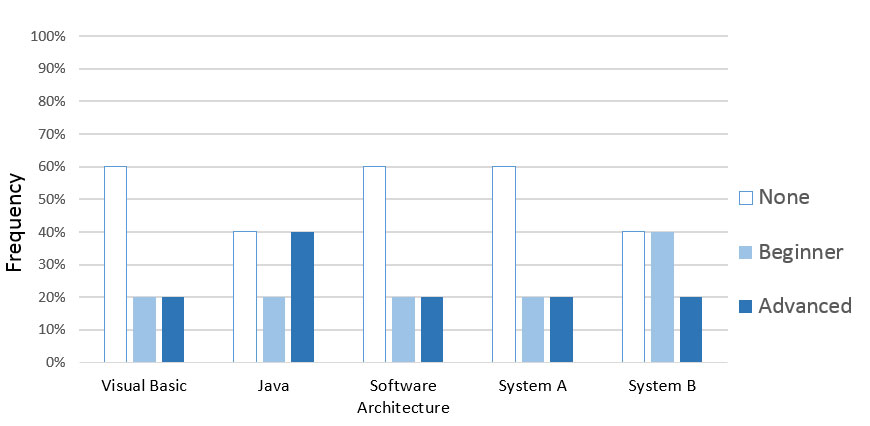
\includegraphics[scale=0.25]{6_expertise_participantes_grupo_1_en}
	\caption{Participants expertise in Group 1.}
%	\label{conhecimentoGrupo1}
 \end{subfigure}
 ~
 \begin{subfigure}[t]{0.5\textwidth}
	\centering
	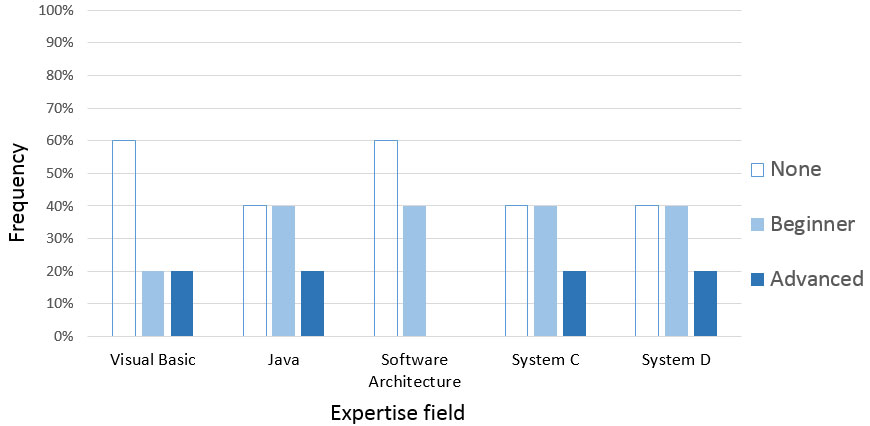
\includegraphics[scale=0.25]{6_expertise_participantes_grupo_2_en}
	\caption{Participants expertise in Group 2.}
 \end{subfigure}
\caption{Expertise of the participants.}
\label{fig:participantes}
\end{figure*}

%Figure \ref{conhecimentoGrupo2} details information about the level of knowledge of 
%participants in Group 2.

%% \begin{figure}[!h]
%% 	\centering
%% 	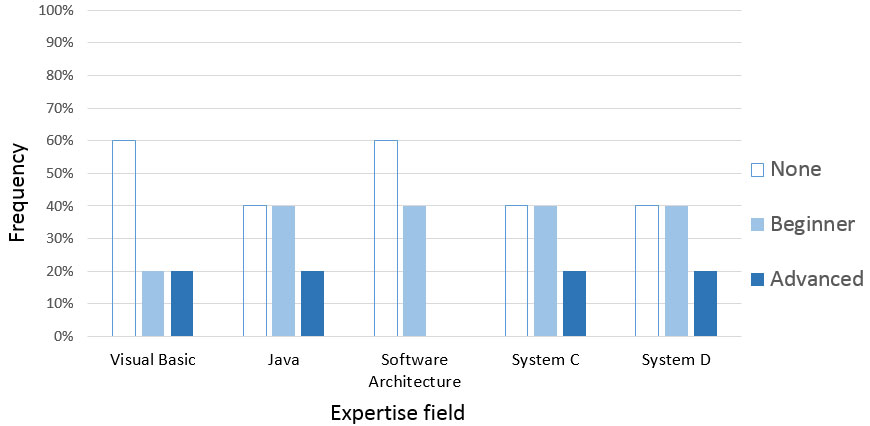
\includegraphics[width=0.45\textwidth]{6_expertise_participantes_grupo_2_en}
%% 	\caption{Participants expertise in Group 2.}
%% 	\label{conhecimentoGrupo2}
%% \end{figure*}

\added[remark={seria importante descrever quais s\~{a}o 
as vari\'{a}veis envolvidas, e quais fatores precisam / est\~{a}o 
sendo controlados com esse design. como os grupos foram formados? 
talvez uma leitura do artigo SoSyM ajude.}]
{As explained}, the subjects were divided into two groups. 
Participants in Group 1 started the extraction in a Visual Basic system 
using the clustering technique. The results of this extraction was collected. Then 
we presented the second technique (a semi-automatic visualization tool) 
and requested the subjects to produce a second model, 
applying both techniques. Afterwards, the same procedure was applied to the Java systems, 
but on the reverse order, i.e, first using a software visualization tool and then clustering. 
For the participants in Group 2, the same procedure applied, but starting with the 
software visualization technique.

%% \begin{figure}[!h]
%% 	\centering
%% 	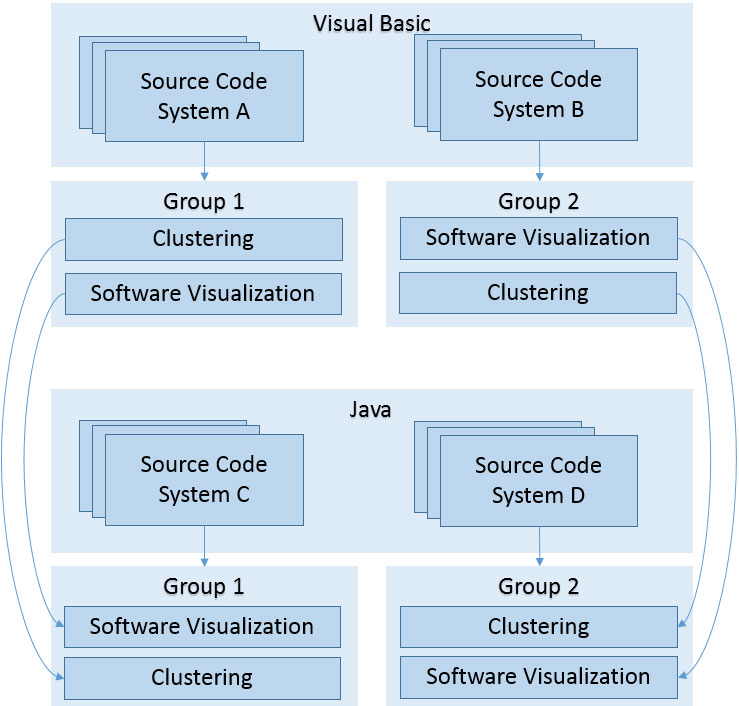
\includegraphics[width=0.43\textwidth]{design_experimento}
%% 	\caption{Design of the experiment.}
%% 	\label{design_experimento}
%% \end{figure}


\subsection{Execution}%
Architecture recovery is an interpretive and interactive process involving many activities. 
Therefore, it may be a time consuming task. For this reason, the experiment seeks to recover the overall 
modular decomposition of the systems architecture. So, for each participant, the basic architecture concepts were introduced, 
as well as the essential elements for detecting the overall architecture of the object systems. 

The semi-automatic analysis of the Visual Basic system was carried out using the 
\texttt{VBDepend} tool. This tool provides several mechanisms that facilitates the exploitation of the system 
architecture in Visual Basic language based on visualization via dependency graphs and dependency structure matrix. 
Figure  \ref{matrizDependenciaVBDependend} highlights a dependency structured  matrix (DSM)~\cite{Tekinerdogan_2009} 
obtained using \texttt{VBDepend} 
tool. 

% TODO: talvez levar esse texo para a secao de background.

% In this case, the DSM is useful for analyzing the properties of complex applications. 
% In an architectural analysis, the couplings between the architectural modules are described and various operations on the matrix can be performed in order to identify architectural relations \cite{Tekinerdogan_2009}.

\begin{figure}[!h]
	\centering
	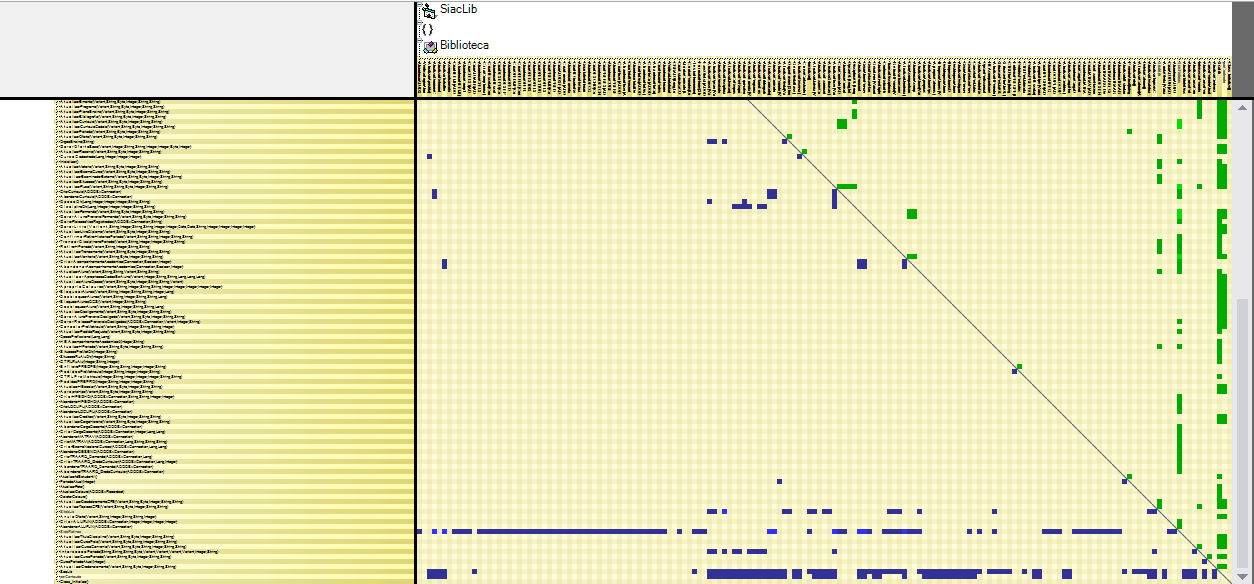
\includegraphics[width=0.45\textwidth]{6_matrizDependenciaVBDependend}
	\caption{Dependency matrix obtained through the use of VBDepend tool.}
	\label{matrizDependenciaVBDependend}
\end{figure}

To analyse the Java systems, the subjects used two different tools: \texttt{ X-Ray} and \texttt{Architexa}. 
The X-Ray software visualization tool is an open source software available as a plug-in for the Eclipse IDE. 
Through this tool, one can get different visions of class-package dependencies and systemic complexity views on Java projects. 
An example of a systemic complexity view can be seen in \ref{xray_complexidade}. In this kind of view, classes are represented 
by rectangles; the width of the rectangles representing the number of methods implemented in a particular class, 
while the height of the rectangle represents the number of lines of code in the class. 
The bonding edge is the relationship between the classes. The nodes can be set as a vertical tree, highlighting the hierarchy of classes.

\begin{figure}[!h]
	\centering
	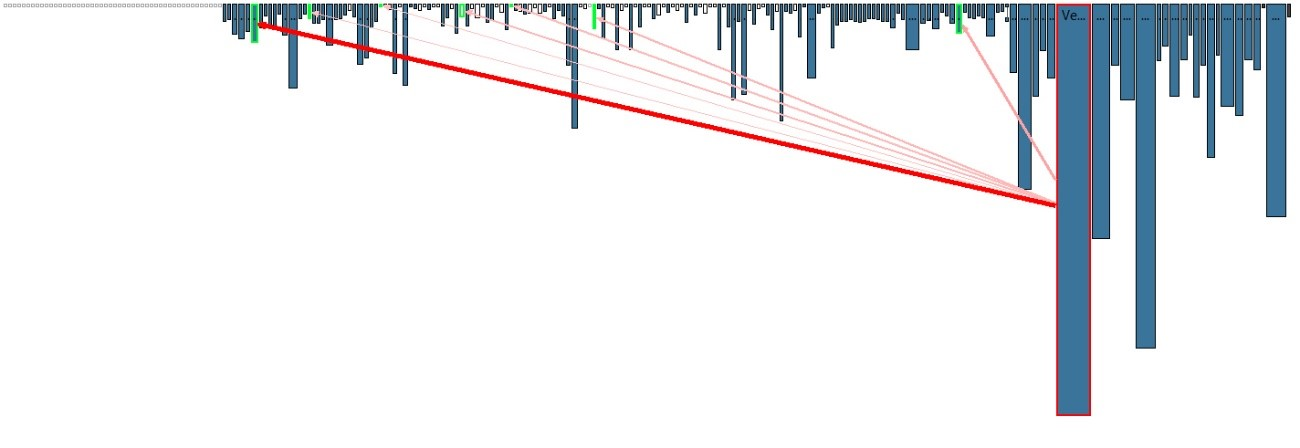
\includegraphics[width=0.45\textwidth]{6_xray_complexidade}
	\caption{Extracted systemic complexity view of a system in Java.}
	\label{xray_complexidade}
\end{figure}

Another tool used for viewing the source, and available to the participants of the experiment is the \texttt{Architexa}. With this tool it is possible to create different diagrams from the static analysis of the code. It is also available as a plug-in for the Eclipse IDE. Using this tool, the participants of the experiment can explore different aspects of the source code, such as a diagram of layers, as in Figure \ref{diagrama_architex}. The diagram layers groups classes based on their respective directories or packages and illustrates the dependency relationships between them. Also, different metrics can be used to highlight important aspects of the system, for example, the rectangle representing the software entities. Software entities that contain a large amount of code are represented by rectangles proportional to their size, which facilitates the identification of important aspects of the code structure. When selected a software entity, the visualization tool displays its respective dependencies by means of an arrow which indicates the origin and destination of the link. The thicker the arrow, the higher the correlation between the elements. Moreover, the colors of each rectangle are changed to emphasize the dependencies.


\begin{figure}[!h]
	\centering
	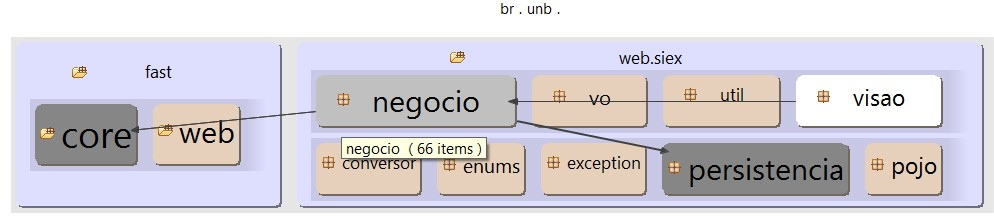
\includegraphics[width=0.45\textwidth]{6_diagrama_architex_2}
	\caption{Extracted systemic complexity view of a system in Java.}
	\label{diagrama_architex}
\end{figure}


The Bunch tool \cite{mitchell_heuristic_2002} was used for clustering approach as the tool is open source and has an intuitive graphical interface, as shown in Figure . Participants in the experiment were instructed to choose between the available algorithms and run the clustering process in the system under analysis. Participants can change the input parameters of the algorithms and run the clustering tool as often as they felt necessary. The process outputs is a file containing the modules automatically mapped by the selected algorithm. Through the output of the analysis, the participants comprised the architectural model of the system under analysis.


\subsection{Results}%

Through the results, calculated from the comparison of the models produced by the participants with models produced by experts in the field, it was possible to investigate the use of architecture recovery approach using clustering and software visualization techniques. 

To analyze the significance of the results, it was used the paired t-test. For this, we observed the different conditions that underpin the paired t-test, as: two related groups; no significant outliers; distribution of the differences in the dependent variable between the two related groups is approximately normally distributed.  Table \ref{tabelaResultadoVB}  describes the comparison data between the scores obtained using one and two techniques. It is possible to see that the average accuracy of the models obnained in Visual Basic sytems using one technique was approximately 51\%, and the average accuracy of the models obtained using two techniques was approximately 77\%. A difference of 26\%. On the other hand,  is possible to note that the mean of the models obtained in Java systems using one technique was approximately 48\%; when used two techniques, the mean was approximately 72\%. A difference of 24\%.

\begin{table}[h]
	\centering
	\caption{Descriptive data table of the systems in Visual Basic and Java.}
	\label{tabelaResultadoVB}
	\resizebox{\columnwidth}{!}{%
	\begin{tabular}{|l|l|l|l|l|l|}
		\hline
		& Technique      & N  & Means & Std. Deviation & Std.Error Mean \\ \hline
		Visual Basic & One Technique  & 10 & 0.517 & 0.091          & 0.028          \\ \hline
		& Two Techniques & 10 & 0.771 & 0.077          & 0.024          \\ \hline
		Java         & One Technique  & 10 & 0.483 & 0.060          & 0.019          \\ \hline
		& Two Techniques & 10 & 0.728 & 0.059          & 0.018          \\ \hline
	\end{tabular}
	}
\end{table}

We now need to analyse if these results are statistically meaningful. We carry out the paired t-test then. Table \ref{tabelaResultadoTesteTVB}, details the paired t-test to compare the results obtained using one technique followed by two techniques. To interpret the results is necessary to observe the Sig. (2-tailed) value, also known as p value. This is the value that determines whether the means are statistically different. If the Sig.(2-tailed) value is greater than 0.05 then there is no statistically significant difference between the two conditions. On the other hand, if the value is less than or equal to 0.05 then there is a statistically significant difference between the two conditions. The significance level of 0.05 reflects the 95\% confidence interval used as parameter value for the calculations.

Analyzing the data for the systems in Visual Basic, it is possible to conclude that there is a significant difference between the scores obtained using one technique (Mean= 0.517, Std. Deviation = 0.091) and two techniques (Mean= 0.771, Std. Deviation= 0.077); t(9)=-10.046, p= 0.000. So, with 95\% confidence, it can be said that there is an increase in results from 0.196 to 0.310 when used two techniques for software architecture recovery. Analyzing the data for the systems in Java language, it is possible to conclude that there is a significant difference between the mean values obtained using one technique (Mean= 0.483, Std. Deviation= 0.060) and two techniques (Mean= 0.728, Std. Deviation= 0.059); t(9)= -10.046, p= 0.000. Thus, with 95\% of confidence, the accuracy improvement varies from 0.207 to 0.283 when used two techniques for software architecture recovery. For the sistems in Java

\begin{table}[h]
	\centering
	\caption{Paired t-test for Visual Basic systems.}
	\label{tabelaResultadoTesteTVB}
	\resizebox{\columnwidth}{!}{%
		\begin{tabular}{|l|l|c|c|c|c|l|l|l|}
			\hline
			& \multicolumn{5}{c|}{Paired  Diferences}                                                                                                                                                                                                             &                              &                         &                                                                                 \\ \cline{2-6}
			&                            & \multicolumn{1}{l|}{}                                    & \multicolumn{1}{l|}{}                                        & \multicolumn{2}{l|}{\begin{tabular}[c]{@{}l@{}}95\% Confidence \\ Interval\end{tabular}} &                              &                         &                                                                                 \\ \cline{5-6}
			& Mean                      & \begin{tabular}[c]{@{}c@{}}Std.\\ Deviation\end{tabular} & \begin{tabular}[c]{@{}c@{}}Std. Error\\ Mean\end{tabular} & Lower                                     & Upper                                     & \multicolumn{1}{c|}{t}       & \multicolumn{1}{c|}{df} & \multicolumn{1}{c|}{\begin{tabular}[c]{@{}c@{}}Sig. \\ (2-tailed)\end{tabular}} \\ \hline
			\begin{tabular}[c]{@{}l@{}}(Visual Basic) \\ One technique-\\ Two techniques \end{tabular} & \multicolumn{1}{c|}{-0.253} & 0.079                                                     & 0.025                                                         & -0.310                                        & -0.196                                        & \multicolumn{1}{c|}{-10.046} & \multicolumn{1}{c|}{9}  & \multicolumn{1}{c|}{0.000}                                                       \\ \hline
			
			\begin{tabular}[c]{@{}l@{}}(Java)\\One technique-\\ Two techniques\end{tabular} & \multicolumn{1}{c|}{-0.245} & 0.053                                                     & 0.0169                                                        & -0.283                                        & -0.207                                        & \multicolumn{1}{c|}{-10.046} & \multicolumn{1}{c|}{9}  & \multicolumn{1}{c|}{0.000}                                                       \\ \hline
				\end{tabular}
	}
\end{table}

After these analyzes, it is possible to conclude that using two techniques produced better results than using only one technique in a software architecture recovery process. Thus, it is possible to answer RQ1, where it is questioned whether the use of both techniques increases the accuracy of the obtained architectural models. Given the above results, it is possible to say that the use of both techniques had a positive impact on the accuracy of the models produced, since all the results indicated an improvement in the accuracy of the models when used the two techniques together.

\replaced{To enhance the results obtained, further analyzes were performed. First, }{To answer RQ2,}, we performed an analysis of the impact on the programming language on the accuracy of the results.  From Table \ref{tabelaOutrasAnalises2} it can be seen that in Visual Basic systems, the average accuracy of the models produced was approximately 60\%. In systems written in Java, the accuracy was approximately 64\%. These values represent the total amount of analyses performed for each language. Since each language was twice analysed in each group, then N equal 20, in this case.

\begin{table}[h]
	\centering
	\caption{Descriptive data table comparing system languages.}
	\label{tabelaOutrasAnalises2}
	\resizebox{\columnwidth}{!}{%
	\begin{tabular}{|l|l|l|l|l|l|}
		\hline
		~         & Language      & N  & Mean   &  Std. Deviation   & Std. Error Mean \\ \hline
		Pair1 & Visual Basic      & 20 & 0.605  & 0.138        & 0.031         \\
		~         & Java           & 20 & 0.644  & 0.153        & 0.034         \\ \hline
	\end{tabular}
	}
\end{table}

To calculate the significance of the means difference and determine if the programming language affects the recovery process, we conducted a paired t-test. The result can be seen in Table \ref{table:test_t3}. Through data analysis, we conclude that there is no significant difference between the mean values of the systems in Visual Basic (Mean= 0.605,  Std. Deviation= 0.138) and Java systems (Mean= 0.644,  Std. Deviation= 0.153); t(19)= -1.867, p= 0.077. \replaced{Given the outcome,}{Thus it is possible to answer RQ2: given the outcome,} we can conclude that, with 95\% of confidence level, the programming languages had no statistically significant effect on the results, since Sig(2-tailed) value is greater than 0.05. So, the difference of means is in the interval (-0.082; 0.004), which includes 0.

\begin{table}[h]
	\centering
	\caption{Paired t-test for the comparison of the two programming languages.}
	\label{table:test_t3}
	\resizebox{\columnwidth}{!}{%
		\begin{tabular}{|l|l|c|c|c|c|l|l|l|}
			\hline
			& \multicolumn{5}{c|}{Paired  Diferences}                                                                                                                                                                                                             &                              &                         &                                                                                 \\ \cline{2-6}
			&                            & \multicolumn{1}{l|}{}                                    & \multicolumn{1}{l|}{}                                        & \multicolumn{2}{l|}{\begin{tabular}[c]{@{}l@{}}95\% Confidence \\ Interval\end{tabular}} &                              &                         &                                                                                 \\ \cline{5-6}
			& Mean                      & \begin{tabular}[c]{@{}c@{}}Std.\\ Deviation\end{tabular} & \begin{tabular}[c]{@{}c@{}}Std. Error\\ Mean\end{tabular} & Lower                                     & Upper                                     & \multicolumn{1}{c|}{t}       & \multicolumn{1}{c|}{df} & \multicolumn{1}{c|}{\begin{tabular}[c]{@{}c@{}}Sig. \\ (2-tailed)\end{tabular}} \\ \hline
			\begin{tabular}[c]{@{}l@{}}Visual Basic-\\ Java\end{tabular} & \multicolumn{1}{c|}{-0.0387} & 0.0928                                                     &  0.020                                                       & -0.082                                      & 0.004                                        & \multicolumn{1}{c|}{-1.867} & \multicolumn{1}{c|}{19}  & \multicolumn{1}{c|}{0.077}                                                       \\ \hline
		\end{tabular}
	}
\end{table}

Finally, it is possible to analyze if the order of the recovery technique affects the results. \deleted{This analysis is useful to check whether starting from visualization or clustering in our process influences the accuracy of the results}. Table \ref{tabelaOutrasAnalises4} details the descriptive results of the data. When using software visualization and then using clustering, the accuracy of the models obtained was approximately 77\%. Moreover, using first the clustering technique then software visualization technique, the accuracy of the models obtained was approximately 72\%.

\begin{table}[h]
	\centering
	\caption{Descriptive data table related to the order of the techniques.}
	\label{tabelaOutrasAnalises4}
	\resizebox{\columnwidth}{!}{%
		\begin{tabular}{|l|l|l|l|l|l|}
			\hline
			~         & Order     						 & N  & Mean   & Std. Deviation   & Std. Error Mean  \\ \hline
			Pair1 & Visualization-Clustering  			  & 10  & 0.771  & 0.077        & 0.024         \\
			~         & Clustering-Visualization          & 10  & 0.728  & 0.059        & 0.018         \\ \hline
		\end{tabular}
	}
\end{table}

To check for the difference between the means, it was conducted a  paired t-test. The results are shown in Table \ref{table:test_t4}. Through data analysis, it is possible to conclude that there is no significant difference between the mean values obtained using Software Visualization prior to Clustering (Mean=0.771,  Std. Deviation= 0.077) and Clustering prior to Software Visualization (Mean= 0.728, Std. Deviation= 0.059); t(9)= 1.456, p= 0.179.

\begin{table}[h]
	\centering
	\caption{Paired t-test for the comparison of the order of techniques.}
	\label{table:test_t4}
	\resizebox{\columnwidth}{!}{%
		\begin{tabular}{|l|l|c|c|c|c|l|l|l|}
			\hline
			& \multicolumn{5}{c|}{Paired  Diferences}                                                                                                                                                                                                             &                              &                         &                                                                                 \\ \cline{2-6}
			&                            & \multicolumn{1}{l|}{}                                    & \multicolumn{1}{l|}{}                                        & \multicolumn{2}{l|}{\begin{tabular}[c]{@{}l@{}}95\% Confidence \\ Interval\end{tabular}} &                              &                         &                                                                                 \\ \cline{5-6}
			& Mean                      & \begin{tabular}[c]{@{}c@{}}Std.\\ Deviation\end{tabular} & \begin{tabular}[c]{@{}c@{}}Std. Error\\ Mean\end{tabular} & Lower                                     & Upper                                     & \multicolumn{1}{c|}{t}       & \multicolumn{1}{c|}{df} & \multicolumn{1}{c|}{\begin{tabular}[c]{@{}c@{}}Sig. \\ (2-tailed)\end{tabular}} \\ \hline
			\begin{tabular}[c]{@{}l@{}}VisualizationClustering-\\ ClusteringVisualization\end{tabular} & \multicolumn{1}{c|}{0.0427} & 0.0927                                                     &  0.029                                                       & -0.023                                      & 0.109                                        & \multicolumn{1}{c|}{1.456} & \multicolumn{1}{c|}{9}  & \multicolumn{1}{c|}{0.179}                                                       \\ \hline
		\end{tabular}
	}
\end{table}

\deleted{Given the above, it is possible to answer RQ3, whether the order of the technique applied can affect the results.} Facing the results, we can say that there is no statistical evidence to say that the order of the approach had an influence on the results, since Sig(2-tailed) value is greater than 0.05 resulting the interval (-0.023, 0.109) which includes 0.

\subsection{Internal validity}%

All participants of the experiment have experience in analysis and development of software systems, which contributes to the representation of the group of analysts and system developers who may require an architectural reconstruction process. The participants of the two experimental groups have similar characteristics.

The use of two programming languages, Visual Basic and Java, contributes to the representation of an organizational environment in which there is no homogeneity in relation to the programming language used by the systems in the company. Despite the fact that the participants are separated into two groups and run the experiment in different objects systems, recovery approach was conducted in systems with similar architectures. Due to this similarity, it is expected that the results are not influenced by the programming language objects, or difference between the systems.

\subsection{External validity}%
The size in LOC and the complexity of the systems objects can influence the generalization of the results. However, such systems present complexity and size similar to most of the systems developed to meet sectorial needs of an organization. 

Also, the limited number of participants of the experiment can not allow a generalization of the experiment. However, through the separation method of the group at random, it was expected to decrease the confusion factor.

\subsection{Discussion}

The experimental study observed the impact of using data clustering and software visualization techniques in the understanding of software systems architecture.

First, it was examined whether the use of software visualization and clustering techniques together improves the accuracy of the architecture recovery process. The results showed that, when used one after the other technique, the accuracy of the models produced had a significant increase. This is because the techniques act in a complementary manner by providing additional information. Also, the use of both techniques together provided to the participants a different perspective of the software, not perceived or not represented when compared to using only a technique. Thus, allowing for recovery of the architecture more accurately. 

Second, an analysis was performed to verify if programming language can affect the recovery of the architecture. The results showed that the programming language had no significant effect on the results. This demonstrates the flexibility of clustering  and software visualization techniques. This flexibility is due to the fact that currently there are several software visualization tools available, which enable the analysis of different programming languages. Also, the clustering approach, implemented by Bunch tool, is designed to be independent of language, since it is only necessary to set up a MDG containing the dependency relationships between the entities of the source code, and this is achieved through static analysis techniques of the source code.

Finally, we observed that the order of execution of the techniques does not significantly affect the results. This indicates that there is no specific order for the application of the techniques in the approach. This was also confirmed by the feedback from participants. When asked about the preference of the order of execution of techniques, some preferred to start with clustering, while others, with the visualization. Thus, the execution of techniques can happen in a subjective way that best meets the needs of the responsible for the recovery of architecture.



